\documentclass[11pt]{article}

\usepackage[utf8x]{inputenc}
\usepackage[slovene]{babel}

\usepackage{amssymb}
\usepackage{amsmath} 

\usepackage[pdftex]{graphicx} % za slike

\title{\textbf{Surface Reconstruction}}
\author{O\v zbolt Menegatti\\
		Anej Placer\\
		Jurij Slabanja}
\date{}
\begin{document}

\maketitle

\section{Opis problema}

Cilj projekta je bil rekonstruirati povr"sino iz oblaka to"ck s pomo"cjo topolo"skih konceptov kot so "Cechov in Vietoris-Rips kompleks ter alfa oblike. Potrebno je bilo vizualizirati rezultate in izra"cunati nekatere topolo"ske invariante kot so homologija in Eulerjeva karakteristika. V nadaljevanju tega poglavja na kratko opi"semo te topolo"ske koncepte.

\subsection{"Cech kompleks}
Izmed implementiranih metod je "Cechov kompleks eden najbolj osnoven. "Ce imamo oblak to"ck, si lahko predstavljamo, da ga naredimo tako, da okoli vsake to"cke o"crtamo navidezno kroglo s polmerom $\delta$. Na podlagi teh krogel to"cke pove"zemo v simplekse in sicer tako, da pove"zemo to"cke katerih krogle imajo neni"celni presek. Na primer "ce imamo dve krogli, ki se sekata, potem moramo njuni sredi"s"ci (njuni to"cki v oblaku to"ck) povezati v 1-simplex oz. rob. "Ce imamo tri krogle, ki se sekajo ena z drugo vendar ne vse hkrati, dobimo prazen trikotnik. "Ce je presek vseh treh krogel neni"celen dobimo polni trikotnik itd. 

Problem s "Cechovim kompleksom je, da je potrebno zelo pazljivo izbrati $\delta$ parameter, saj lahko zelo hitro dobimo visoko dimenzijske simplekse, kar ni vedno za"zeljeno. Do istega problema pride, "ce oblak to"ck ni homogeno porazdeljen, ampak so to"cke ponekod bolj gosto posejane. V takih delih oblaka tudi zelo hitro dobimo visoko dimenzijske simplekse.

\subsection{Vietoris-Rips}
Vietoris-Rips kompleks je v osnovi zelo podoben "Cechovemu kompleksu, vendar tu ne operiramo ve"c z navideznimi kroglami ampak z radaljami med pari to"ck. Za Vietoris-Ripsa velja, da je nek simpleks del kompleksa, "ce je premer simpleksa manjsi ali enak $2\delta$. Razliko s "Cechom se najla"zje vidi, "ce vzamemo za oblak to"ck ogli"s"ca enakostrani"cnega trikotnika in za $\delta$ parameter pribli"zno polovico dol"zine stranice, kot je prikazano na Sliki~\ref{fig:vrdiag}. S "Cechovim kompleksom dobimo samo prazni trkotnik, medtem ko z Vietoris-Ripsom dobimo poln 2-simpleks.

\begin{figure}[!htb]
    \centering
    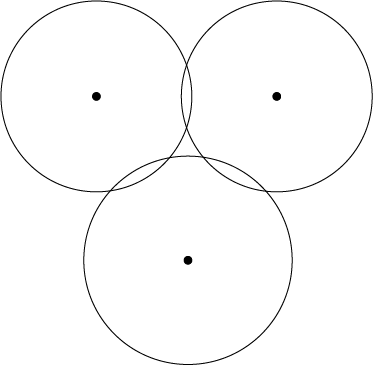
\includegraphics[width=0.4\textwidth]{vrdiag.png}
    \caption{Z Vietoris-Ripsom dobimo polni trikotnik, za razliko od "Cechovega kompleksa, kjer dobimo praznega}
    \label{fig:vrdiag}
\end{figure}

Izka"ze se, da si lai"cno lahko Vietoris-Ripsa razlagamo kot "Cechov kompleks, pri katerem so dodani simpleksi, ki imajo vsa svoja lica vklju"cena v "Cechovem kompleksu. Iz tega sledi, da je "Cechov kompleks podmno"zica Vietoris-Ripsovega kompleksa. Seveda naj opomnimo, da morata pri tem imeti Vietoris-Rips in "Cechov kompleks enak parameter $\delta$. 

Prav tako kot "Cechov kompleks ima tudi Vietoris-Rips probleme z visoko dimenzijskimi simpleksi.

\subsection{Alpha oblike}

Alfa oblike izbolj"sajo "ze omenjena kompleksa v oziru dimenzionalnosti generiranih simpleksov. V osnovi se gre za to, da "cez oblak to"ck nari"semo Voronojev diagram nato pa pove"zemo samo to"cke, ki so so Voronojevske sosede in so med sabo oddaljene za manj kot $\delta$ (podobno kot pri prej"snjih dveh kompleksih). Dve tocki sta Voronojevski sosedi, "ce si Voronojevski celici, katerima to"cki pripadata, delita vsaj eno to"cko t.j. celici se dotikata. Ker povezujemo samo Voronojevske sosede, so alfa oblike podmno"zica Delaunayjeve triangulacije, kar pomeni da bojo imele geometrijsko realizacijo v neki $\mathbb{R}^{d}$ in bo dimenzionalnost simpleksov nizka. 

\subsection{Homologija}

Bistvo algebraične topologije so homološke grupe. Topologijo predstavimo z Bettijevimi števili, ki predstavljajo rang homoloških grup. Homologija stopnje 0 predstavlja povezanost podatkov (koliko posameznih povezanih komponent imamo), homologija stopnje 1 detektira luknje in tunele, homologija stopnje 2 votline, itd. V tej nalogi smo se omejili na te glavne tri grupe. 

Povezanost diskretnih točk predstavimo s kompleksi. Povezanost je odvisna od določenih parametrov, npr. radij okoli točk, ki pove s katerimi drugimi točkami so le-te povezane. Ideja je podobna pri vseh treh obravnavanih kompleksih. Iz tega sledi, da je povezanost nekih diskretnih točk odvisna od izbranih parametrov in univerzalnega odgovora ni. 

Ta problem rešujemo s \emph{persistenco}. Ideja persistence je, da se z večanjem radija okoli točk spreminjajo kompleksi in homološke grupe. To pa nam pove katera topologija skozi spremembe \emph{persistira}.

Iz slike~\ref{homo} je razvidno, da z večanjem radija  postaja graf bolj povezan. Črte v prikazanem diagramu predstavljajo ``življensko dobo'' povezane komponente. Pri neki delti (epsilon) število presekanih črt predstavlja bettijevo število za določeno stopnjo.

\begin{figure}[htb]
    \centering
    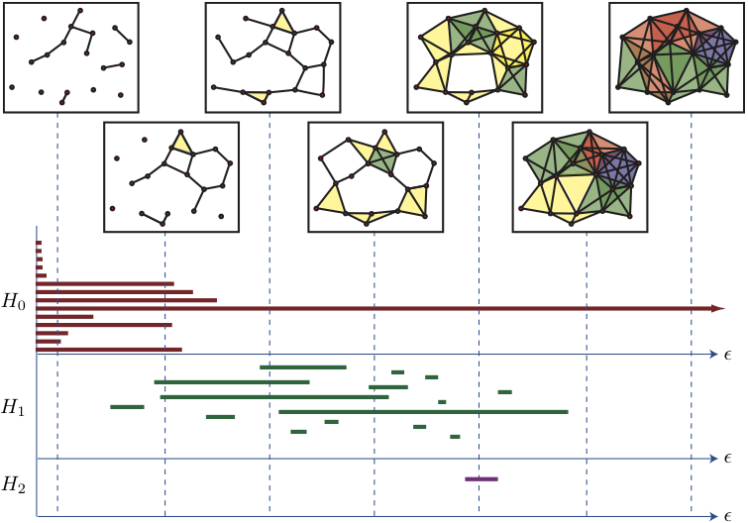
\includegraphics[width=0.8\textwidth]{homo.png}
    \caption{Persistenca in barkoda.}
    \label{homo}
\end{figure}

Če pogledamo drugi primer je prečrtanih 6 povezanih komponent in 2 luknji. V seminarski nalogi smo prav tako za posamezen kompleks zgenerirali zgoraj opisano persistenčno tabelo, kjer se filtrira ven vse vnose (začetek/konec), ki vsebujejo delto (torej smo presekali črto).

\subsection{Euler}

\section{Pristop}

Uporabili smo knji"zico Dyonisus za izra"cun topologij in knji"zico QT za izris in nadzor aplikacije. Implementirali smo ve"c pristopov, Vietoris-Rips kompleks, Alfa oblike ter "Cechov kompleks. Izkazalo se je, da je "Cech izjemno po"casen, tako da je bil kasneje odstranjen, "se vedno pa ga lahko najdete v zakomentiranem delu kode.

Za prikaz imamo ve"c opcij, prosojnost pogleda, izris povezav in izbor oblaka to"ck. Za potrebe naloge smo implementirali tudi mo"znost izbire parametra $\delta$ ter procenta izbranih to"ck na kompleksu.

\section{Te"zave}

Te"zave smo imeli z ve"c detajli, a izpostavimo dva:

\begin{enumerate}
\item "Cechove metode nam ni uspelo z omejenim pomnilnikom izvesti v normalnem "casu.
\item Alpha oblike so druga"cne, kot na vajah. Namre"c v strukturi data ne najdemo podatkov o dol"zini povezave, da bi lahko uspe"sno filtrirali za dan delta. Problem smo rocno zaob"sli, vendar re"sitev ne dela optimalno.
\end{enumerate}

\section{Rezultati}

Z večanjem $\delta$ seveda narašča čas računanja. Alpha oblike delujejo hitreje kot vietoris-rips. Zelo zanimivo (in pravilno) je delovanje izračuna homologije, saj npr. pri krogli, v primeru, da ima ta 3 luknje, izračuna homologijo kot (1,2,0), torej 1 povezana komponenta in 2 tunela. V primeru, da imamo 4 luknje dobimo homologijo (1,3,0), torej 3 tuneli oz. če sploščimo dobljeno formacijo okol ene od lukenj dobimo 3 luknje (glej Sliko~\ref{lukne}).

\begin{figure}[htb]
    \centering
    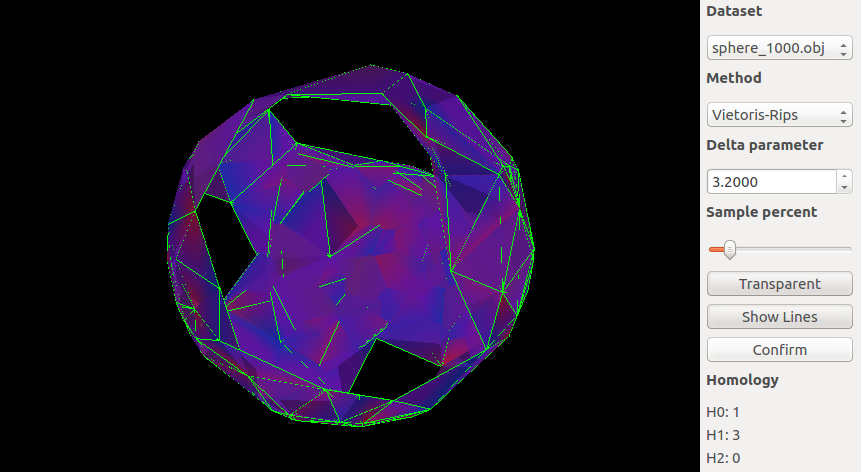
\includegraphics[width=1\textwidth]{lukne_primer.png}
    \caption{Primer homologije pri krogli s 4 luknjami.}
    \label{lukne}
\end{figure}

$\delta$ parameter je tesno povezan s tipom podatkov. Pri gostejših oblakih bo zadostila manjša $\delta$. Podobno so lahko razdalje v setu točk zelo velike (čeprav je oblak zelo velik oz. gost), zato bo potrebna večja $\delta$. Iz slik v nadaljevanju je vidno delovanje programa. Program je prilo"zen v zip datoteki.

\begin{figure}[htb]
    \centering
    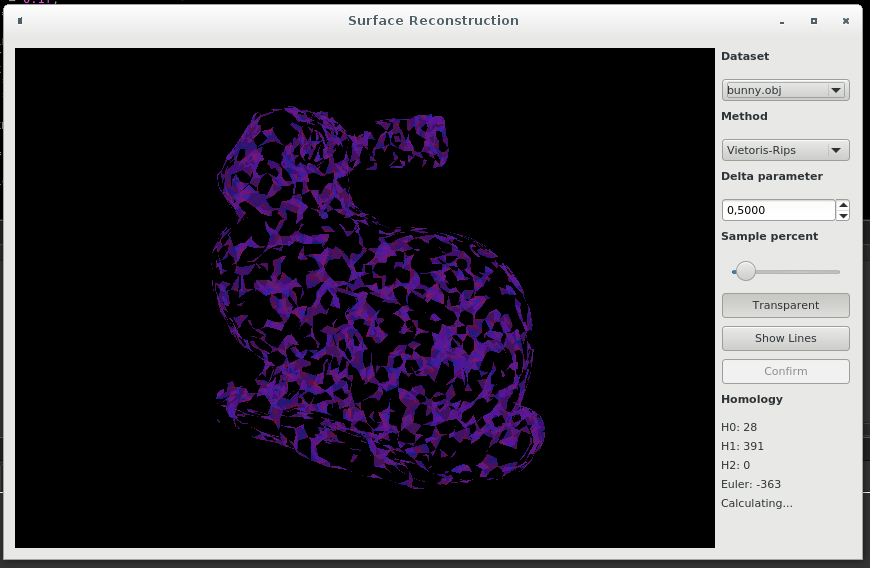
\includegraphics[width=1\textwidth]{vr_long.png}
    \caption{Izra"cun Vietoris-Ripsa s premajhnim delta}
    \label{fig:vr1}
\end{figure}


\begin{figure}[htb]
    \centering
    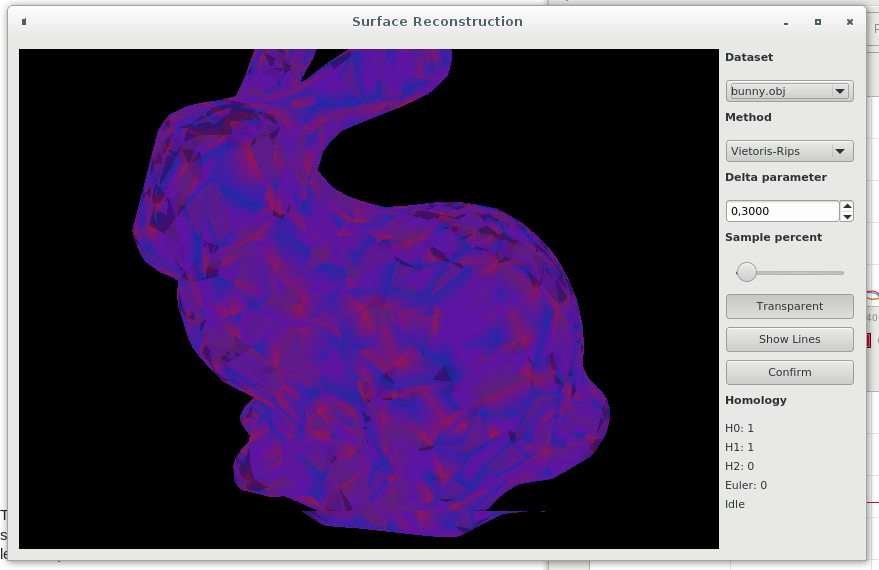
\includegraphics[width=1\textwidth]{vr_full_9639823.png}
    \caption{Izra"cun Vietoris-Ripsa z zadostnim delta, vendar malo to"ckami. "St. to"ck: 9639823}
    \label{fig:vr2}
\end{figure}

\begin{figure}[htb]
    \centering
    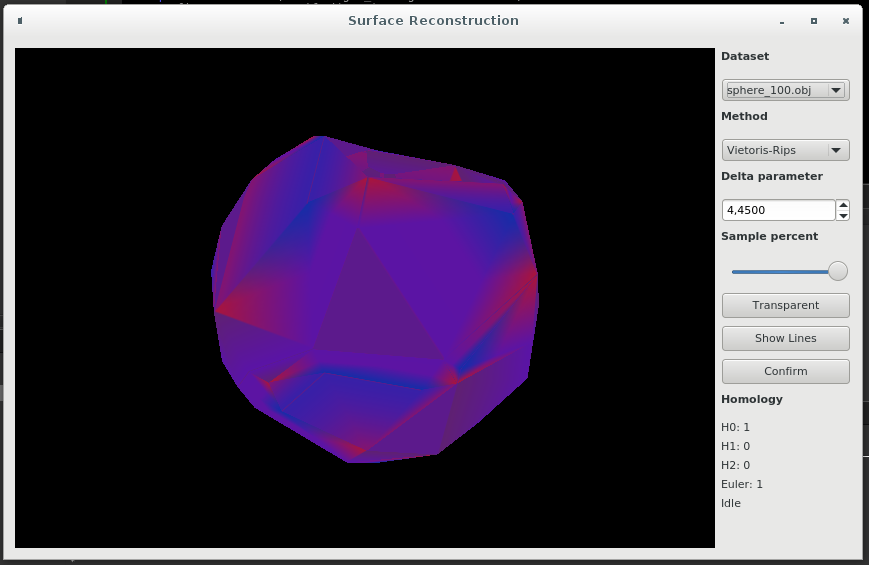
\includegraphics[width=1\textwidth]{vr_1hole.png}
    \caption{Izra"cun Vietoris-Ripsa n krogli: ena luknja}
    \label{fig:vr3}
\end{figure}

\begin{figure}[htb]
    \centering
    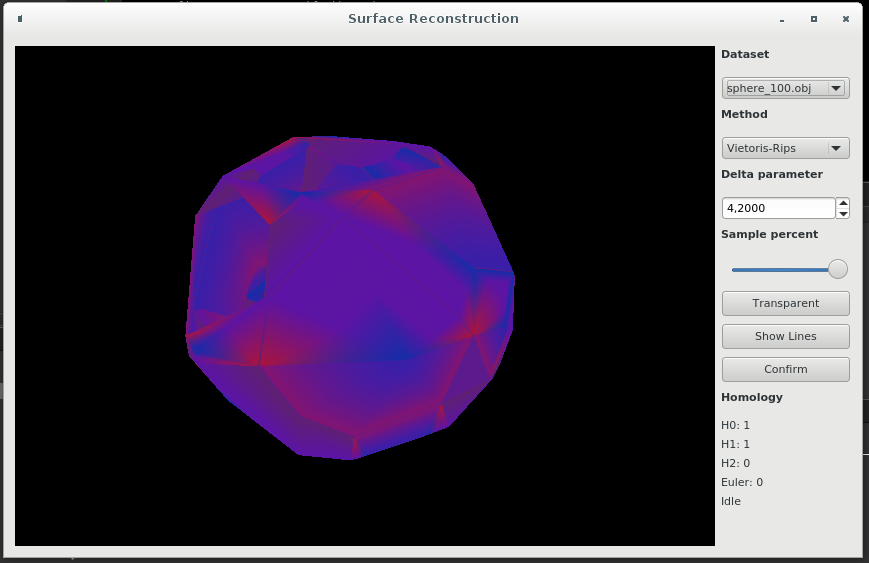
\includegraphics[width=1\textwidth]{vr_2hole.png}
    \caption{Izra"cun Vietoris-Ripsa n krogli: dve lunkji}
    \label{fig:vr4}
\end{figure}

\begin{figure}[htb]
    \centering
    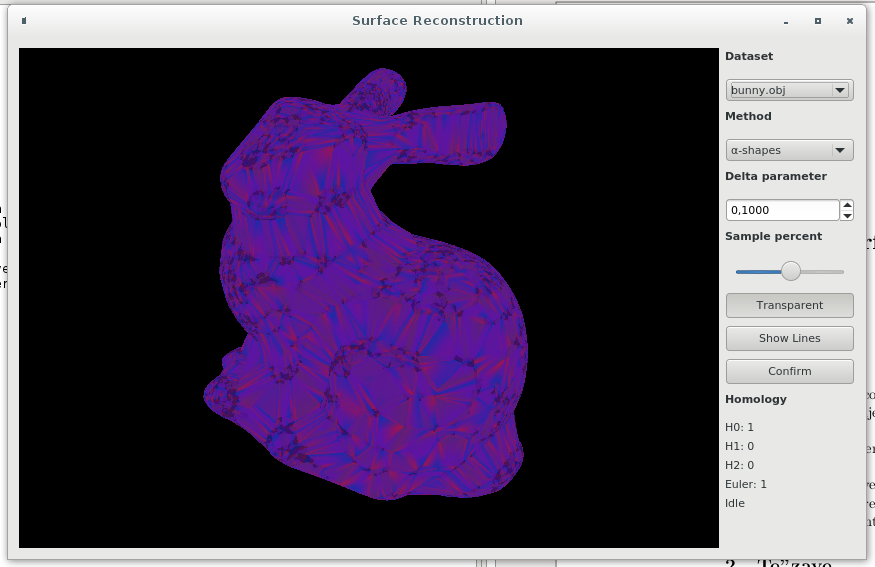
\includegraphics[width=1\textwidth]{alpha_full.png}
    \caption{Izra"cun $\alpha$-oblik: polno, ena lunkja na dnu zajca}
    \label{fig:a1}
\end{figure}

\begin{figure}[htb]
    \centering
    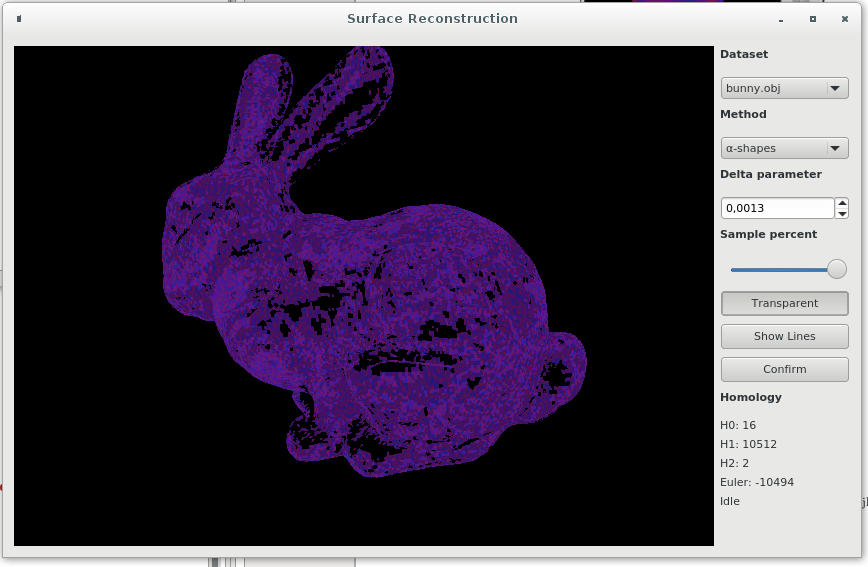
\includegraphics[width=1\textwidth]{alpha_lowdelta.png}
    \caption{Izra"cun $\alpha$-oblik: polno, Izra"cun na vseh to"ckah, a s premajhnim $\delta$}
    \label{fig:a1}
\end{figure}

\begin{figure}[htb]
    \centering
    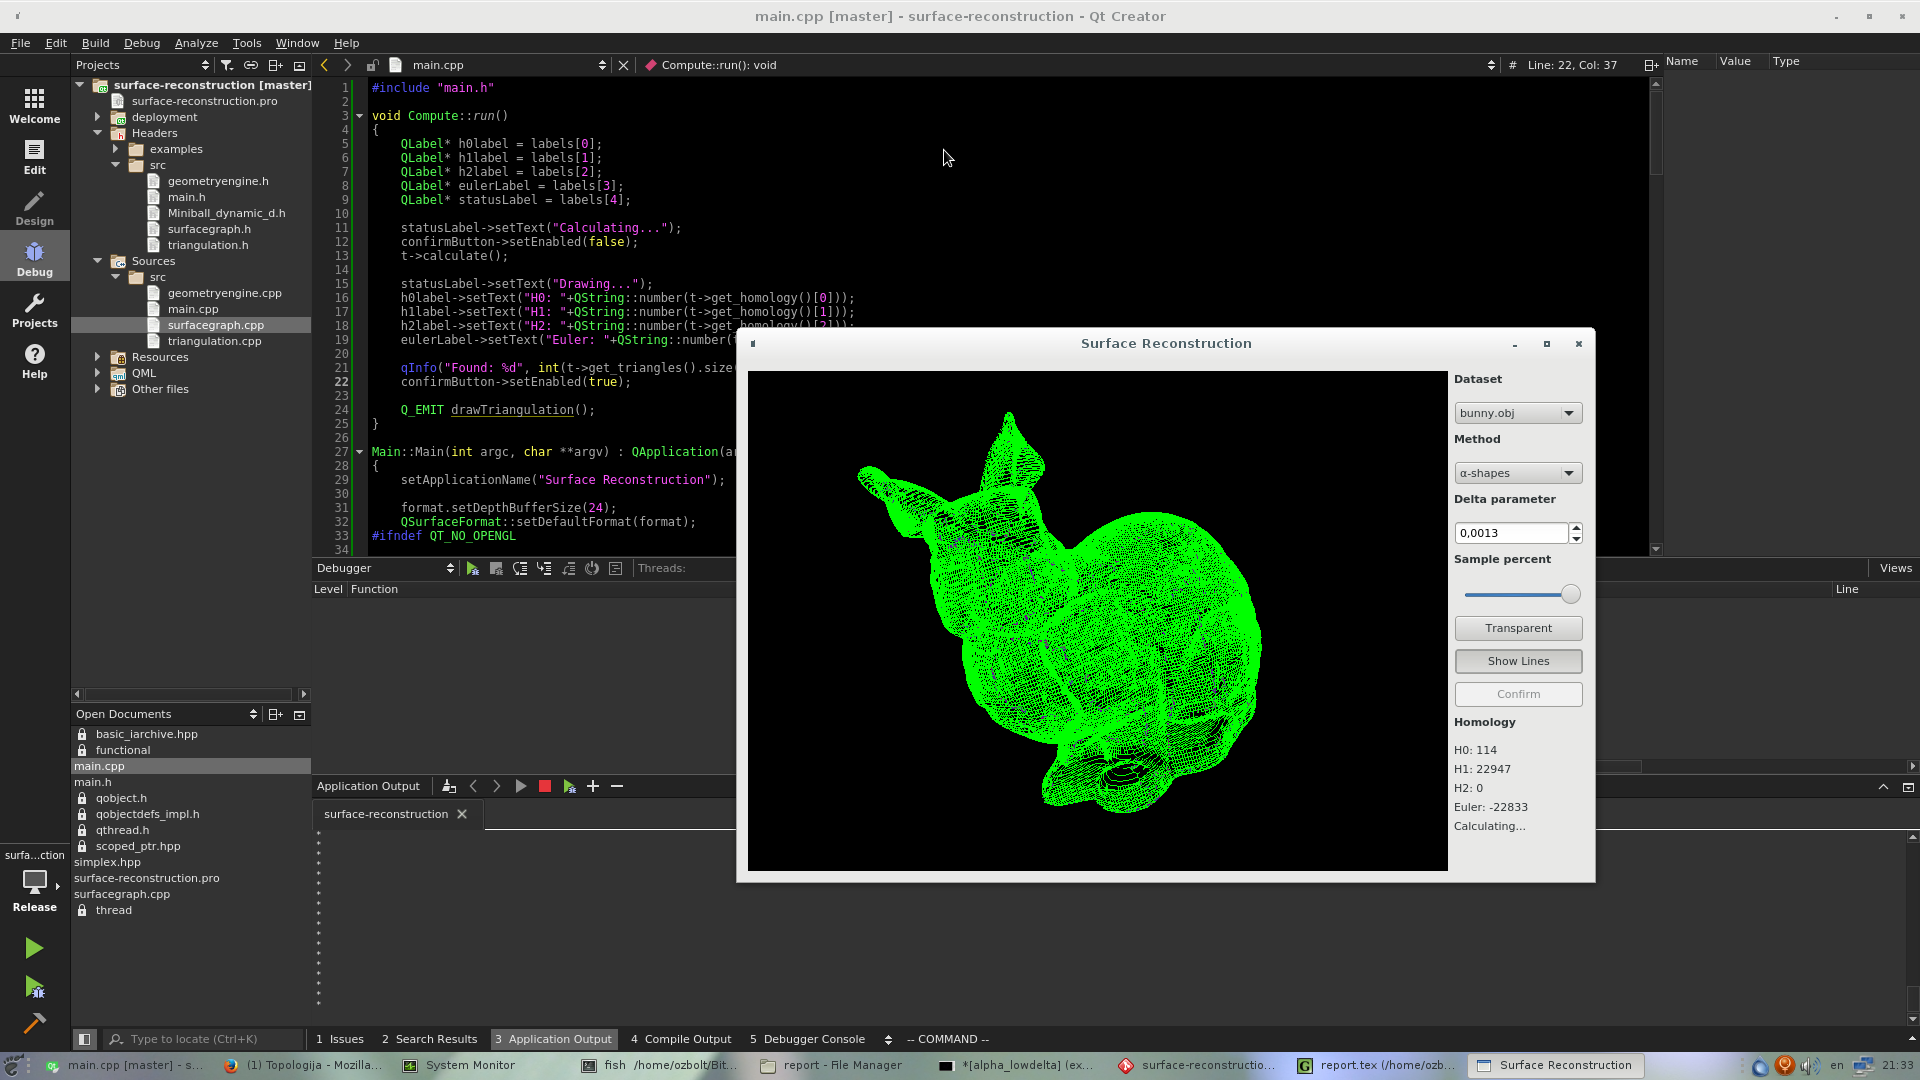
\includegraphics[width=\textwidth]{lines.png}
    \caption{Prikaz povezav}
    \label{fig:edges}
\end{figure}

%\newpage % mogoce nav treba

\section{Delitev dela}

\subsection{Ožbolt}
Alpha shapes, branje in formatiranje podatkov, testiranje. 

\subsection{Anej}
Vietoris-Rips, homologija, izris crt, shaderji.

\subsection{Jurij}
Cech, euler, večina grafičnega vmesnika, osnoven izris.

\end{document}
